\section{Automatisierung der Datenerfassung}\label{sec:Datenerfassung}
Allgemein l�sst sich sagen, dass bei der Wissensbasiserweiterung ein hybrides Modell sinnvoll dass eine Kooperation zwischen einem menschlichen Experten und automatisierten Methoden darstellt. Die Autoren in \cite{tecuci1994} weisen ebenso darauf hin, dass manuelle und maschinelle Wissenserschlie�ung jeweils eigene St�rke haben, die in einem hybriden Ansatz kombiniert werden k�nnen\cite[S.137]{tecuci1994}.\\
In Bezug auf die Wissensbasisentwicklung k�nnen folgende Phasen unterschieden werden \cite[S.1444]{tecuci1992}: 
\begin{itemize}
\item[1.] Systematische Erfassung vom Expertenwissen
\item[2.] Verfeinerung der Wissensbasis
\item[3.] Reorganisation der Wissensbasis
\end{itemize}
Die erste Phase umfasst die Festlegung der grunds�tzlichen Struktur der Wissensbasis, die im Rahmen eines indirekten Wissenserwerbs stattfindet. Das strukturierte Interview wird dabei oft eingesetzt \cite[S.1444]{tecuci1992}. Das Ergebnis der ersten Phase ist eine initiale Wissensbasis, die unvollst�ndig und teilweise falsch ist. In der zweiten Phase wird die initiale Wissensbasis mithilfe der geeigneten Datenerfassungsmethoden solange erweitert und verbessert, bis sie vollst�ndig und korrekt genug ist, um ein gegebenes Problem richtig zu l�sen. In der dritten Phase wird die vollst�ndige und korrekte Wissensbasis reorganisiert, um die Effizienz der L�sungsberechnung zu steigern \cite[S.1445]{tecuci1992}. Zusammenfassend lassen sich die Phasen in der Abbildung \ref{drei_phasen} darstellen: 
\begin{figure}[H] 
	\centering
	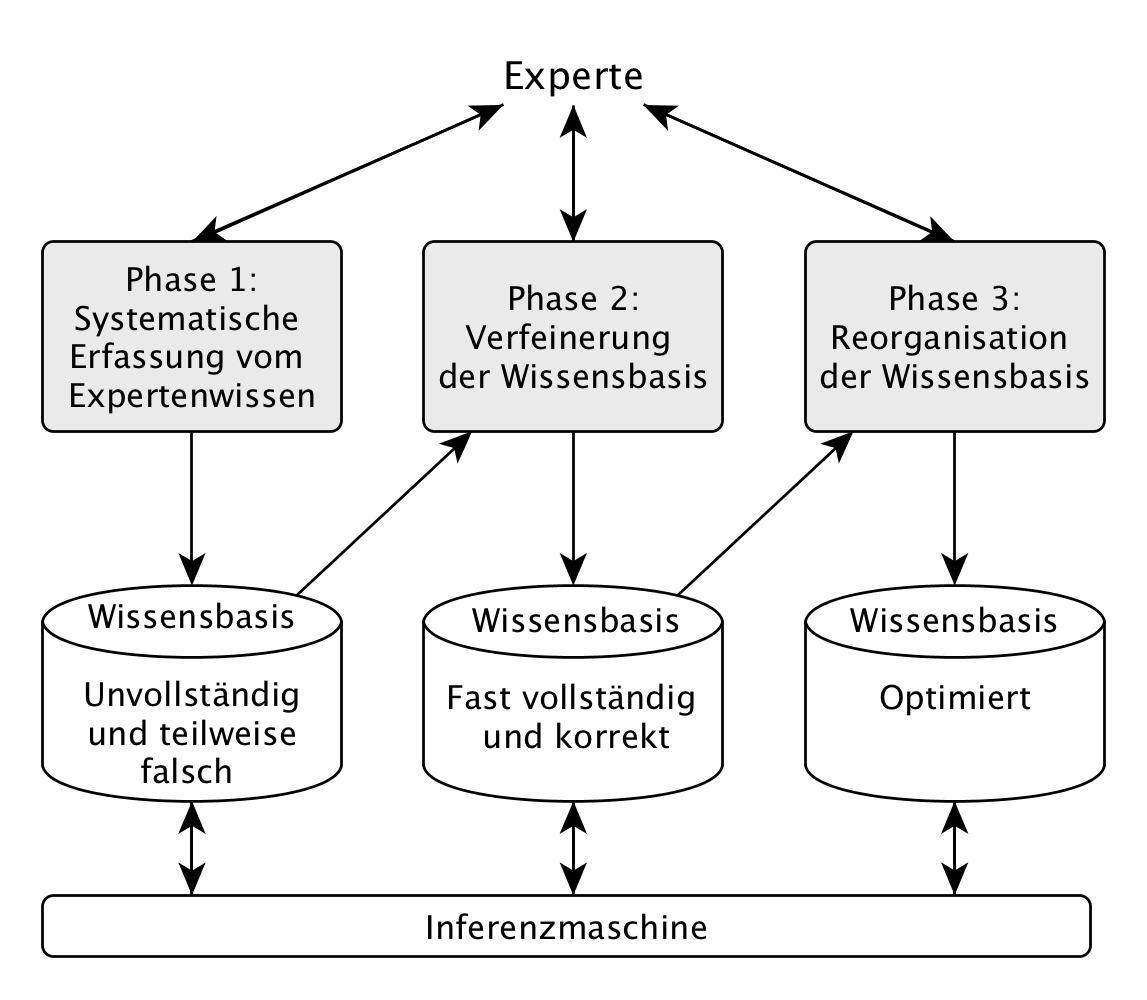
\includegraphics[width=0.65\textwidth]{images/drei_phasen.png}
	\caption{Phasen der Expertensystementwicklung, \cite[S.138]{tecuci1994}}
	\label{drei_phasen}
\end{figure}
Die Methoden der Automatisierung der Datenerfassung, die im weiteren Verlauf behandelt werden, beziehen sich auf die zweite Phase der Wissensbasisentwicklung.

\subsection{Die Wissenstr�gerschnittstelle}
Stark an die Arbeit von \cite{gebus2009} orientiert.

\subsection{Maschineller Wissenserwerb}
Eine Auswahl an generellen Methoden

\subsection{Schnittstelle f�r Validierung und Speicherung}
Zweck, Konzept